%%This is a very basic article template.
%%There is just one section and two subsections.
\documentclass{article}

\usepackage{graphicx}
\usepackage{listings}
\usepackage{color}

\definecolor{listinggray}{gray}{0.9}
\definecolor{lbcolor}{rgb}{0.9,0.9,0.9}
\lstset{
    keywordstyle=\bfseries\ttfamily\color[rgb]{0,0,1},
    identifierstyle=\ttfamily,
    commentstyle=\color[rgb]{0.133,0.545,0.133},
    stringstyle=\ttfamily\color[rgb]{0.627,0.126,0.941},
    showstringspaces=false,
    basicstyle=\tiny,
    numberstyle=\tiny,
    framexleftmargin=3pt,
    numbers=left,
    stepnumber=1,
    numbersep=15pt,
    tabsize=2,
    breaklines=true,
    prebreak = \raisebox{0ex}[0ex][0ex]{\ensuremath{\hookleftarrow}},
    breakatwhitespace=false,
    aboveskip={1.5\baselineskip},
    columns=fixed,
    upquote=true,
    extendedchars=true,
  	frame=l,
    sensitive=true,
}

\renewcommand{\thesection}{Task \arabic{section}}
\renewcommand{\thesubsection}{\arabic{section}.\arabic{subsection}}

\title{TDT4205 Compilers\\
\Huge Exercise 1}
\author{Stian Hvatum (hvatum)\\MTDT}

\begin{document}
\maketitle

\section{}
Version info of \emph{gcc}, \emph{flex} and \emph{bison}
\begin{itemize}
  \item gcc (GCC) 4.2.3 (Ubuntu 4.2.3-2ubuntu7)
  \item flex 2.5.34
  \item bison (GNU Bison) 2.3
\end{itemize}


\section{}
A lexical analyzer is a program that accepts the source code of a program as a
stream of characters, and identifying them as lexemes and outputs this as
tokens.

An acceptor is a program or machine that inputs something, like the
token stream generated by the lexical analyzer, and desides if it satisfies a
given syntax, like a programming language. If the input is accepted, the
acceptor returns \emph{true}, else it returns \emph{false}.
\newpage
\section{}
\subsection{}
\begin{figure}[h]
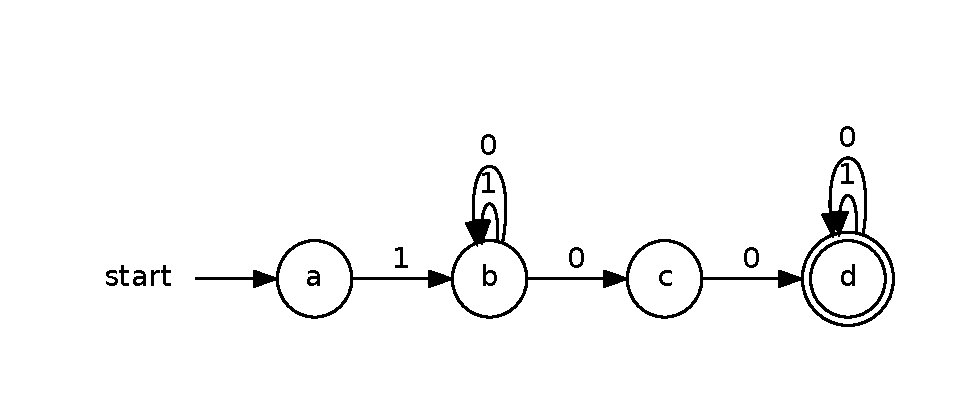
\includegraphics[width=327px]{NDFA31.pdf}
\caption{NDF for 1(0|1)*00(0|1)*}
\end{figure}

\subsection{}
This language includes:
\begin{itemize}
  \item The word 100
  \item All words starting with 100
  \item All words starting with 1 and ending with 00
  \item All words starting with 1 and containing 00
\end{itemize}
given the alphabeth is the set of {0 1}

Examples are 
\begin{itemize}
  \item 1111111111111111100111111111111111111
  \item 10011111111111111111111
  \item 10011001100110011001
  \item 10001
\end{itemize}

\newpage

\subsection{}
\begin{figure}[h]
\begin{tabular}{|l||c|c|c|c|}
\hline
 & a & b & c & d\\
\hline
\hline
1 & b & b & - & d\\
0 & - & \{b c\} & d & d \\
\hline
\end{tabular}
\caption{Transition table for 1(0|1)*00(0|1)*}
\end{figure}
\section{}
\begin{figure}[h]
\centerline{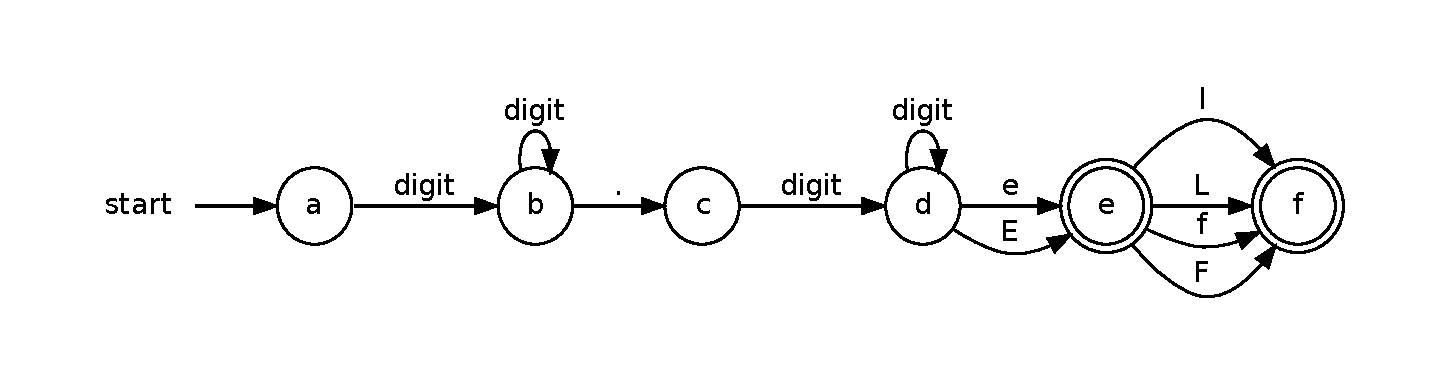
\includegraphics[width=427px]{NDFA4.pdf}}
\caption{DFA for float}
\end{figure}
\newpage
\section*{Appendix}
\subsection*{DOT-code for NDFA 3.1}
\lstinputlisting{NDFA31.gv}
\newpage
\subsection*{DOT-code for NDFA 4}
\lstinputlisting{NDFA4.gv}
\end{document}
